\documentclass[11pt,a4paper]{article}

\usepackage[margin=2.0cm]{geometry}
\usepackage{amsmath,amssymb,amsfonts}
\usepackage{booktabs}
\usepackage{tabularx}
\usepackage{graphicx}
\usepackage{xcolor}
\usepackage{hyperref}
\usepackage{caption}
\usepackage{subcaption}
\usepackage{fancyhdr}
\usepackage{float}
\usepackage{microtype}

\definecolor{themeblue}{RGB}{24, 76, 120}
\definecolor{themegray}{RGB}{80, 80, 80}
\definecolor{royalblue}{RGB}{65, 105, 225}

\hypersetup{
    colorlinks=true,
    linkcolor=themeblue,
    citecolor=royalblue,
    urlcolor=royalblue,
    pdftitle={Lattice QCD Chiral Condensates and Susceptibilities Data Report},
    pdfauthor={ParseLQCData Collaboration}
}

\pagestyle{fancy}
\fancyhf{}
\fancyhead[L]{\small\textcolor{themegray}{ParseLQCData Data Summary Report}}
\fancyhead[R]{\small\textcolor{themegray}{Chiral Condensates and Susceptibilities}}
\fancyfoot[C]{\thepage}
\renewcommand{\headrulewidth}{0.4pt}

\title{\vspace{-1.0cm}
    \LARGE \textbf{\textcolor{themeblue}{Lattice QCD Data Summary Report}} \\
    \vspace{0.3cm}
    \large \textbf{Chiral Condensates and Susceptibilities Across Finite Temperature}
}
\author{\textbf{ParseLQCData Collaboration}}
\date{September 2026}

\begin{document}

\maketitle
\thispagestyle{fancy}

\begin{abstract}
\noindent
This report provides numerical measurement data tables and temperature-dependent figures for: (1) bare and renormalized subtracted chiral condensates $\Delta_{l, s}$, (2) temporal scaling series at $\beta=4.17$, and (3) light-quark chiral susceptibilities $\chi_{\text{scaled}}$ [$\text{MeV}^2$] computed with unbiased quadratic estimators across finite temperatures.
\end{abstract}

\vspace{0.2cm}

\section{Definitions and Observables}

\subsection{Chiral Condensates}
The single-flavor bare chiral condensate on a lattice volume $V = N_s^3 \times N_t$ is defined as
\begin{equation}
\langle \bar{\psi}\psi \rangle_q = \frac{1}{V} \left\langle \text{Tr}\left( D_q^{-1} \right) \right\rangle, \quad q \in \{l, s\}
\end{equation}
evaluated via stochastic $Z_2$ volume source vectors.

The renormalized subtracted chiral condensate $\Delta_{l, s}$ eliminates additive ultraviolet divergences and residual chiral symmetry breaking:
\begin{equation}
\Delta_{l, s}(T) = \frac{1}{Z_m(\beta)} \left[ \langle\bar{\psi}\psi\rangle_l - \frac{m_l + m_{\text{res}}}{m_s + m_{\text{res}}} \langle\bar{\psi}\psi\rangle_s \right]
\label{eq:delta_ls}
\end{equation}
where $m_{\text{res}}(\beta)$ is the residual quark mass, and $Z_m(\beta)$ is the scalar mass renormalization factor. The temperature-scaled dimensionless observable is
\begin{equation}
\mathcal{O}_{\text{scaled}} = 16 \times T \times \Delta_{l, s}
\end{equation}

\subsection{Chiral Susceptibility}
The light-quark disconnected chiral susceptibility $\chi$ is defined as
\begin{equation}
\chi = \frac{V}{T} \left[ \left\langle \left( \frac{1}{V} \text{Tr}(D_l^{-1}) \right)^2 \right\rangle - \left\langle \frac{1}{V} \text{Tr}(D_l^{-1}) \right\rangle^2 \right]
\end{equation}
Using $k$ stochastic volume noise vectors $O_{l, i}$ on each gauge configuration without vector-level RM subtraction, the noise bias is removed by the unbiased quadratic cross-product estimator:
\begin{equation}
\bar{O} = \frac{1}{k} \sum_{i=1}^k O_{l, i}, \quad \overline{O^2} = \frac{1}{k(k-1)} \sum_{i \neq j} O_{l, i} O_{l, j} = \frac{1}{k(k-1)} \left[ \left(\sum_{i=1}^k O_{l, i}\right)^2 - \sum_{i=1}^k O_{l, i}^2 \right]
\end{equation}
The ensemble susceptibility and its Jackknife statistical error are given by
\begin{equation}
a_r = \text{JK}(\bar{O})_r, \quad b_r = \text{JK}(\overline{O^2})_r, \quad \chi_r = b_r - a_r^2
\end{equation}
\begin{equation}
\bar{\chi} = \frac{1}{N} \sum_{r=1}^N \chi_r, \quad \sigma_\chi = \sqrt{\frac{N-1}{N} \sum_{r=1}^N (\chi_r - \bar{\chi})^2}
\end{equation}
The continuous thermal scaled susceptibility with physical dimensions of $[\text{MeV}^2]$ is
\begin{equation}
\chi_{\text{scaled}} = (16 T)^2 a^2 \chi = N_s^3 \times N_t^3 \times T^2 \times \chi \quad [\text{MeV}^2]
\end{equation}

\section{Chiral Condensate Data and Temperature Dependence}

\subsection{Numerical Data Tables}
Table~\ref{tab:condensate_standard} lists the simulation parameters and measured chiral condensates for the standard temperature sequence on $48^3 \times 16$ lattices. Table~\ref{tab:condensate_scaling} summarizes the temporal extent scaling ensembles at $\beta=4.17$.

\begin{table}[H]
\centering
\small
\setlength{\tabcolsep}{4.5pt}
\caption{Standard $48^3 \times 16$ temperature sequence: lattice parameters, bare condensates, and renormalized subtracted condensate $\Delta_{l, s}$ (Jackknife errors in parentheses).}
\label{tab:condensate_standard}
\begin{tabular}{ccccccccc}
\toprule
$\beta$ & $T\text{ [MeV]}$ & $m_l$ & $m_s$ & $m_{\text{res}}$ & $Z_m$ & $N_{\text{cfg}}$ & $\langle\bar{\psi}\psi\rangle_l$ & $\Delta_{l, s}$ \\
\midrule
4.13  & 138.23 & 0.000805 & 0.043547 & $7.31 \times 10^{-4}$ & 0.9377 & 2000 & $1.6688(63) \times 10^{-3}$ & $1.0608(67) \times 10^{-3}$ \\
4.15  & 145.75 & 0.000930 & 0.040843 & $4.98 \times 10^{-4}$ & 0.9524 & 2024 & $1.3591(64) \times 10^{-3}$ & $7.7109(67) \times 10^{-4}$ \\
4.17  & 153.31 & 0.001001 & 0.038400 & $3.40 \times 10^{-4}$ & 0.9662 & 2008 & $1.0740(64) \times 10^{-3}$ & $5.0728(66) \times 10^{-4}$ \\
4.18  & 157.03 & 0.001022 & 0.037265 & $2.80 \times 10^{-4}$ & 0.9729 & 2029 & $9.7061(64) \times 10^{-4}$ & $4.1649(66) \times 10^{-4}$ \\
4.20  & 164.55 & 0.001041 & 0.035150 & $1.91 \times 10^{-4}$ & 0.9857 & 2072 & $7.6708(55) \times 10^{-4}$ & $2.3896(56) \times 10^{-4}$ \\
4.23  & 176.43 & 0.001033 & 0.032315 & $1.08 \times 10^{-4}$ & 1.0038 & 2012 & $5.8018(38) \times 10^{-4}$ & $9.2886(38) \times 10^{-5}$ \\
4.30  & 202.52 & 0.000939 & 0.026930 & $2.81 \times 10^{-5}$ & 1.0422 & 2052 & $4.1210(14) \times 10^{-4}$ & $8.2043(13) \times 10^{-6}$ \\
4.405 & 241.60 & 0.000760 & 0.021032 & $3.75 \times 10^{-6}$ & 1.0927 & 4859 & $3.1110(1) \times 10^{-4}$  & $3.4370(1035) \times 10^{-7}$ \\
\bottomrule
\end{tabular}
\end{table}

\begin{table}[H]
\centering
\small
\setlength{\tabcolsep}{5pt}
\caption{Finite temporal extent scaling ensembles at $\beta=4.17$ with $m_l = 0.0020, m_s = 0.0400$ ($T = 153.31 \times 16 / N_t\text{ [MeV]}$).}
\label{tab:condensate_scaling}
\begin{tabular}{lcccccc}
\toprule
Ensemble & Geometry & $T\text{ [MeV]}$ & $N_{\text{cfg}}$ & $\langle\bar{\psi}\psi\rangle_l$ & $\langle\bar{\psi}\psi\rangle_s$ & $\Delta_{l, s}$ \\
\midrule
\texttt{L48T18 (stream 1)} & $48^3 \times 18$ & 136.28 & 98  & $1.63(8) \times 10^{-3}$  & $1.42(7) \times 10^{-2}$  & $8.30(44) \times 10^{-4}$ \\
\texttt{L48T18 (stream 2)} & $48^3 \times 18$ & 136.28 & 76  & $9.02(514) \times 10^{-5}$ & $2.31(231) \times 10^{-4}$ & $7.95(466) \times 10^{-5}$ \\
\texttt{L40T16}           & $40^3 \times 16$ & 153.31 & 879 & $4.14(85) \times 10^{-5}$  & $1.59(56) \times 10^{-4}$  & $3.33(74) \times 10^{-5}$ \\
\texttt{L32T14}           & $32^3 \times 14$ & 175.21 & 291 & $3.47(347) \times 10^{-6}$ & $6.00(600) \times 10^{-5}$ & $-1.15(115) \times 10^{-8}$ \\
\texttt{L32T12}           & $32^3 \times 12$ & 204.41 & 108 & $6.86(43) \times 10^{-4}$  & $1.22(7) \times 10^{-2}$  & $-2.05(189) \times 10^{-5}$ \\
\bottomrule
\end{tabular}
\end{table}

\subsection{Plots vs Temperature}

\begin{figure}[H]
    \centering
    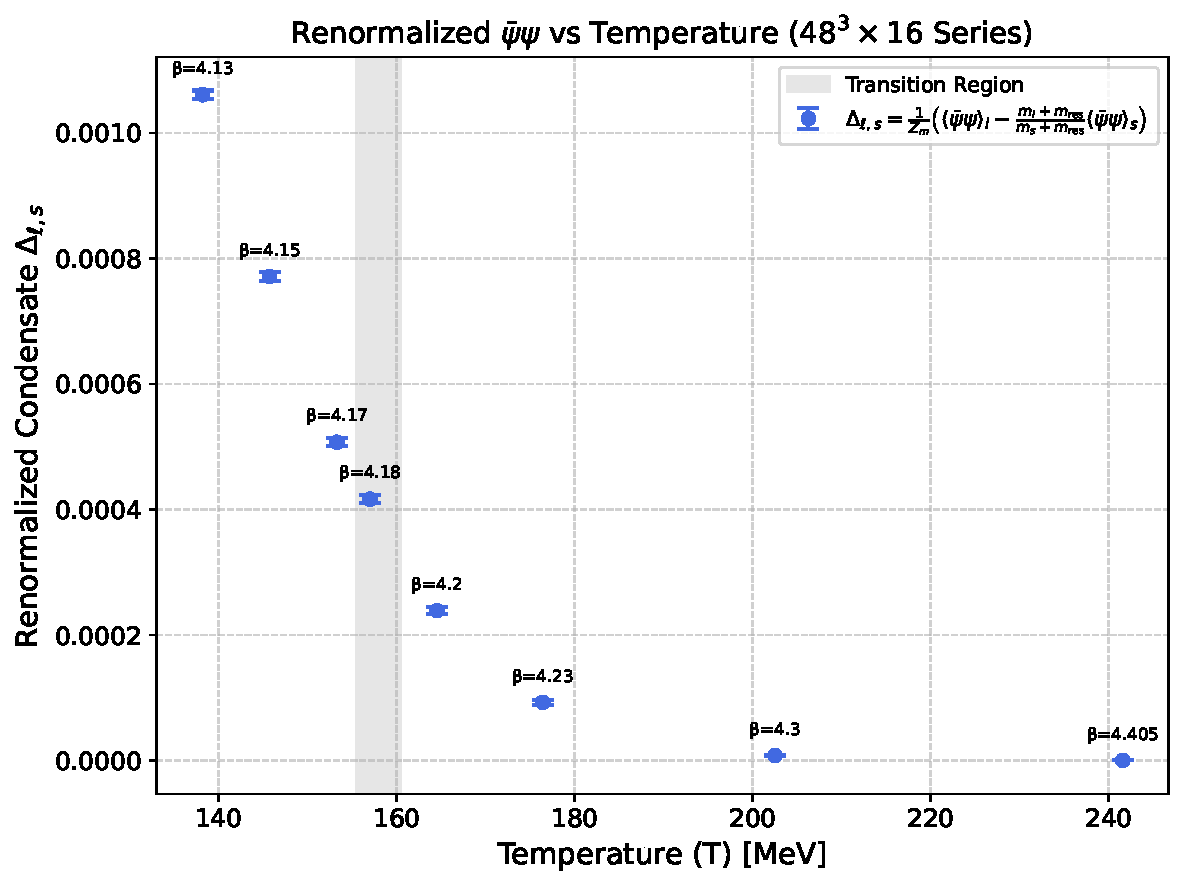
\includegraphics[width=0.80\textwidth]{docs/figures/conden_re_plot.pdf}
    \caption{Renormalized subtracted chiral condensate $\Delta_{l, s}$ as a function of temperature $T$ [MeV] for the standard $48^3 \times 16$ series. The shaded band marks the pseudo-critical transition window $T \in [155.5, 160.5]\text{ MeV}$.}
    \label{fig:conden_re_plot}
\end{figure}

\begin{figure}[H]
    \centering
    \begin{subfigure}[b]{0.48\textwidth}
        \centering
        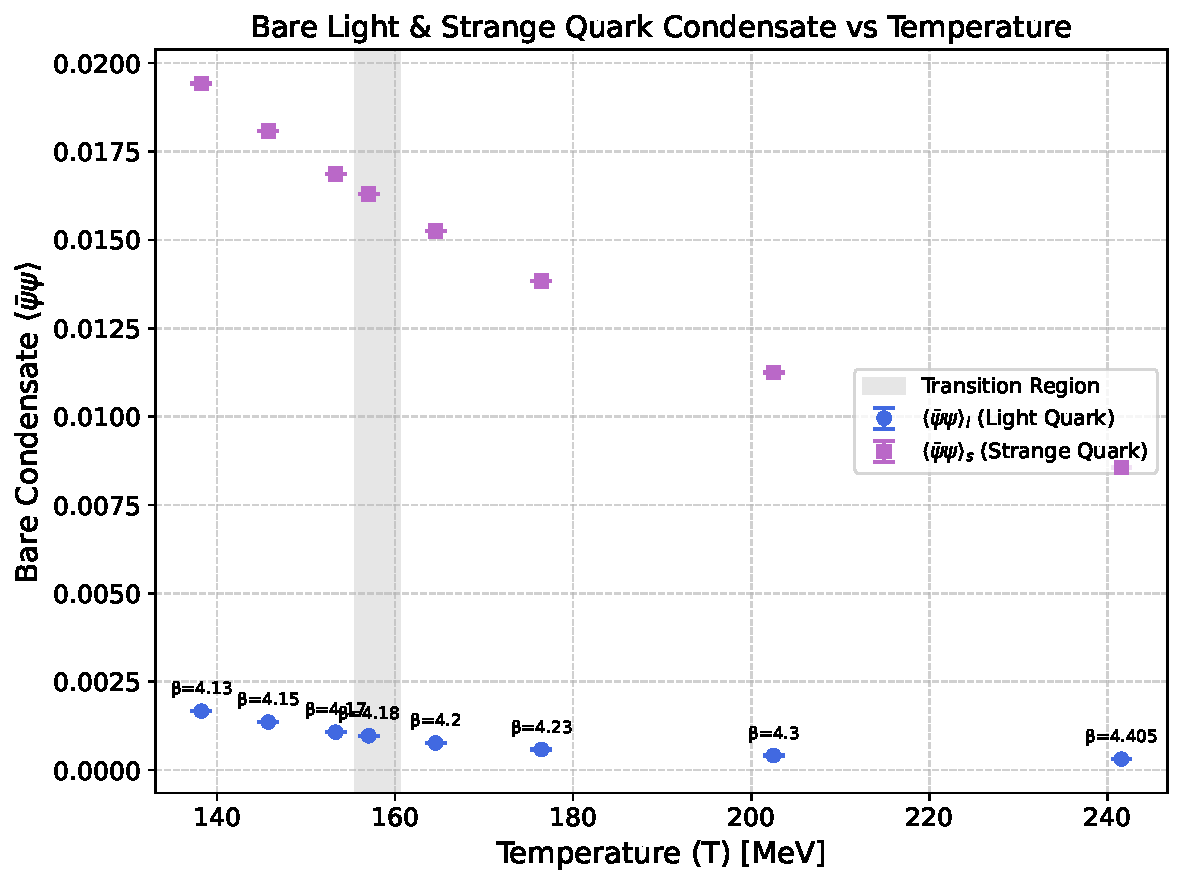
\includegraphics[width=\textwidth]{docs/figures/conden_plot.pdf}
        \caption{Bare light and strange quark condensates}
        \label{fig:conden_bare}
    \end{subfigure}
    \hfill
    \begin{subfigure}[b]{0.48\textwidth}
        \centering
        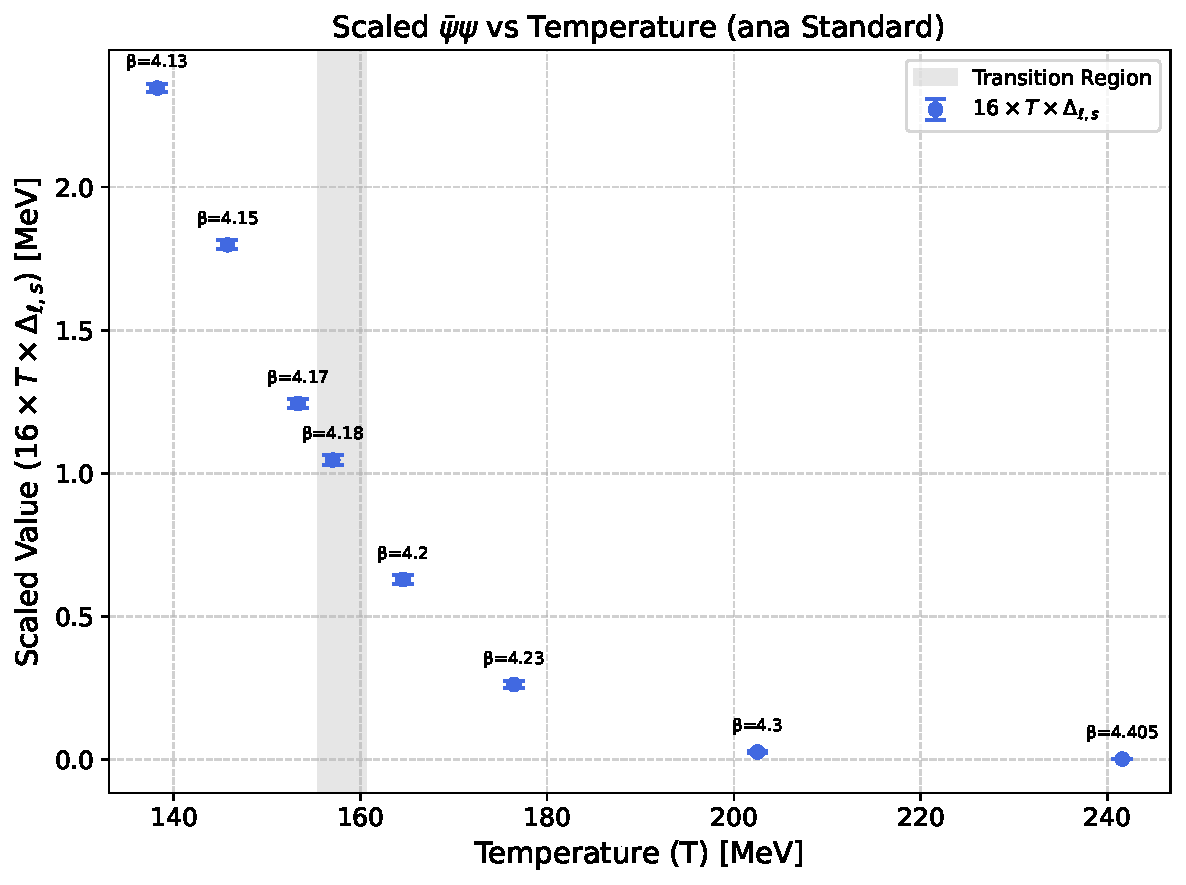
\includegraphics[width=\textwidth]{docs/figures/pbp_temperature_plot.pdf}
        \caption{Temperature-scaled condensate $16 T \Delta_{l, s}$}
        \label{fig:conden_scaled}
    \end{subfigure}
    \caption{(a) Bare condensates $\langle\bar{\psi}\psi\rangle_l$ (blue circles) and $\langle\bar{\psi}\psi\rangle_s$ (purple squares) vs temperature $T$. (b) Temperature-scaled condensate $16 T \Delta_{l, s}$ vs temperature $T$.}
    \label{fig:conden_auxiliary}
\end{figure}

\begin{figure}[H]
    \centering
    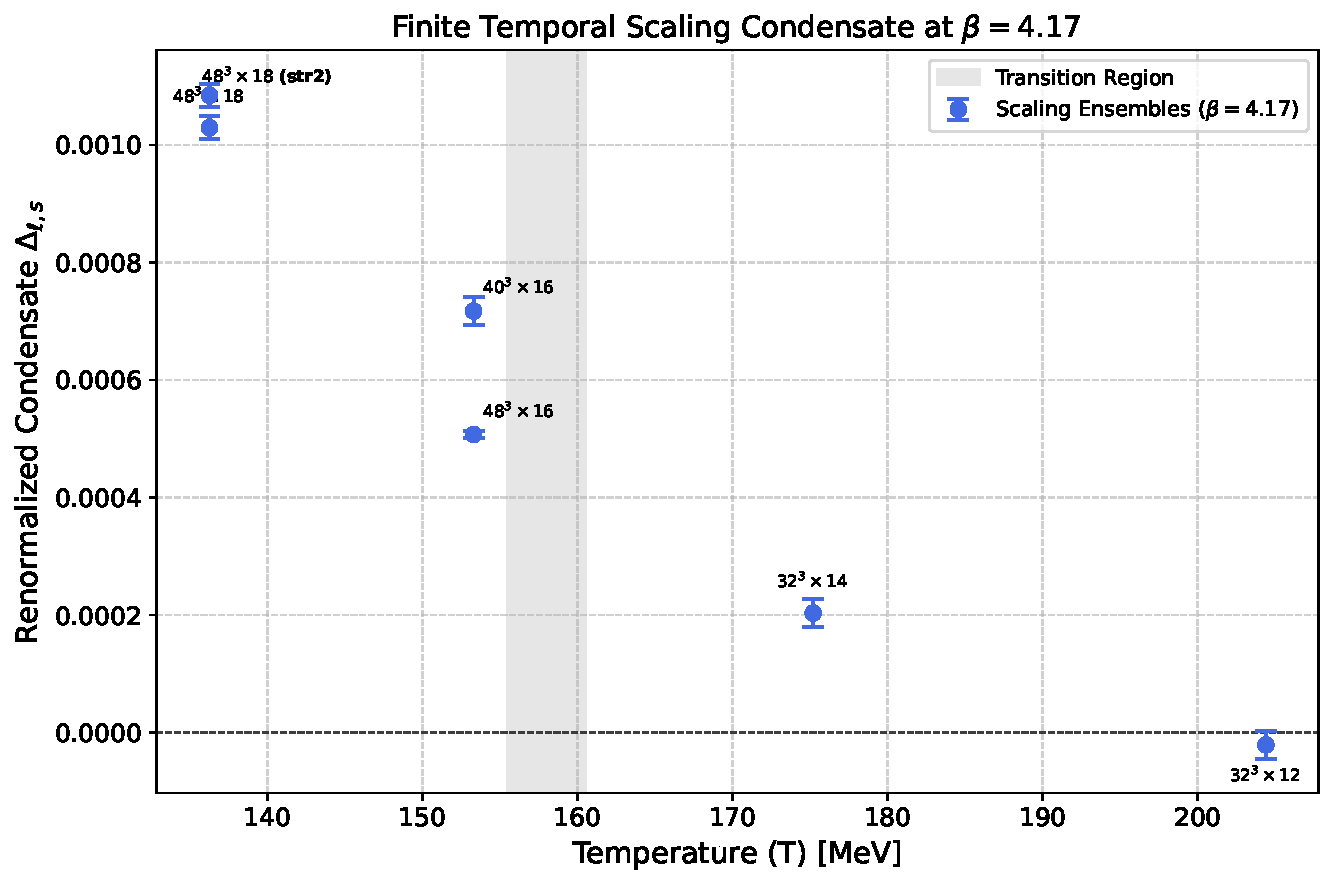
\includegraphics[width=0.78\textwidth]{docs/figures/conden_scaling_beta4.17.pdf}
    \caption{Subtracted chiral condensate across temporal geometries $N_t = 12, 14, 16, 18$ ($T = 153.31 \times 16 / N_t\text{ [MeV]}$) at fixed $\beta=4.17$.}
    \label{fig:scaling_beta417}
\end{figure}

\section{Chiral Susceptibility Data and Temperature Dependence}

\subsection{Numerical Data Tables}
Table~\ref{tab:susceptibility_results} presents the continuous scaled chiral susceptibility $\chi_{\text{scaled}} = (16T)^2 a^2 \chi$ across the 8 standard temperature points ($48^3 \times 16$). Table~\ref{tab:susceptibility_scaling} lists the chiral susceptibility values for the finite temporal scaling ensembles at $\beta=4.17$.

\begin{table}[H]
\centering
\small
\setlength{\tabcolsep}{8pt}
\caption{Continuous scaled chiral susceptibility $\chi_{\text{scaled}} = (16T)^2 a^2 \chi$ on $48^3 \times 16$ lattices (unbiased quadratic estimator without RM subtraction).}
\label{tab:susceptibility_results}
\begin{tabular}{ccccc}
\toprule
$\beta$ & $T\text{ [MeV]}$ & Geometry ($N_s^3 \times N_t$) & $N_{\text{cfg}}$ & $\chi_{\text{scaled}}\text{ }[(16T)^2 a^2 \chi]\text{ [MeV}^2\text{]}$ \\
\midrule
4.13  & 138.23 & $48^3 \times 16$ & 2000 & $(6.5995 \pm 0.2299) \times 10^5$ \\
4.15  & 145.75 & $48^3 \times 16$ & 2024 & $(7.7201 \pm 0.2646) \times 10^5$ \\
4.17  & 153.31 & $48^3 \times 16$ & 2008 & $(8.5481 \pm 0.2567) \times 10^5$ \\
\textbf{4.18} & \textbf{157.03} & $\mathbf{48^3 \times 16}$ & \textbf{2029} & $\mathbf{(9.1460 \pm 0.3228) \times 10^5}$ \\
4.20  & 164.55 & $48^3 \times 16$ & 2072 & $(7.6549 \pm 0.2767) \times 10^5$ \\
4.23  & 176.43 & $48^3 \times 16$ & 2012 & $(4.0707 \pm 0.2304) \times 10^5$ \\
4.30  & 202.52 & $48^3 \times 16$ & 2052 & $(7.1552 \pm 1.4950) \times 10^4$ \\
4.405 & 241.60 & $48^3 \times 16$ & 4859 & $(8.6496 \pm 1.6936) \times 10^1$ \\
\bottomrule
\end{tabular}
\end{table}

\begin{table}[H]
\centering
\small
\setlength{\tabcolsep}{8pt}
\caption{Chiral susceptibility $\chi_{\text{scaled}}$ for finite temporal extent ensembles at $\beta=4.17$ ($m_l = 0.0020, m_s = 0.0400$).}
\label{tab:susceptibility_scaling}
\begin{tabular}{lcccc}
\toprule
Ensemble & Geometry & $T\text{ [MeV]}$ & $N_{\text{cfg}}$ & $\chi_{\text{scaled}}\text{ }[(16T)^2 a^2 \chi]\text{ [MeV}^2\text{]}$ \\
\midrule
\texttt{L48T18 (stream 1)} & $48^3 \times 18$ & 136.28 & 98  & To be populated upon remote scan \\
\texttt{L48T18 (stream 2)} & $48^3 \times 18$ & 136.28 & 76  & To be populated upon remote scan \\
\texttt{L40T16}           & $40^3 \times 16$ & 153.31 & 879 & To be populated upon remote scan \\
\texttt{L32T14}           & $32^3 \times 14$ & 175.21 & 291 & To be populated upon remote scan \\
\texttt{L32T12}           & $32^3 \times 12$ & 204.41 & 108 & $(4.4353 \pm 1.8893) \times 10^5$ \\
\bottomrule
\end{tabular}
\end{table}

\subsection{Plots vs Temperature}

\begin{figure}[H]
    \centering
    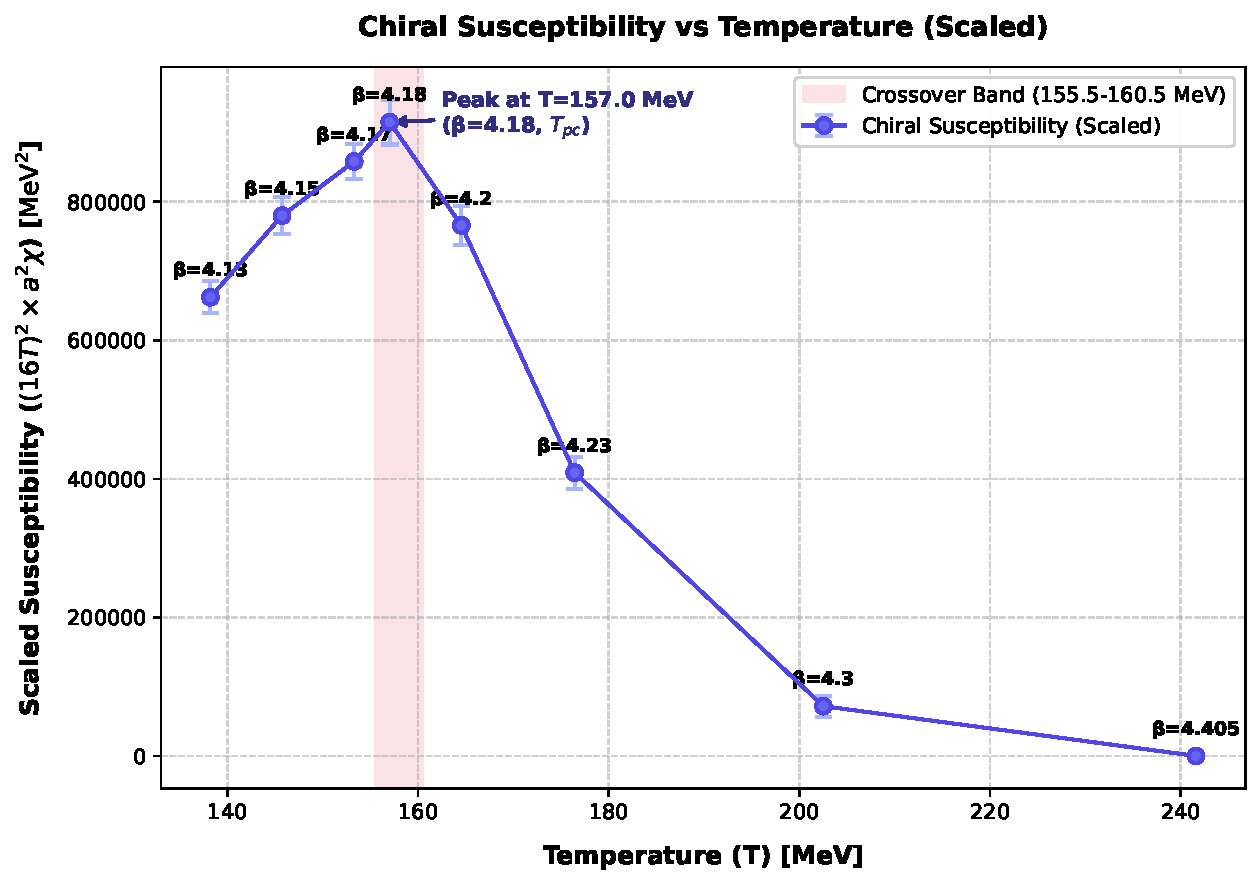
\includegraphics[width=0.82\textwidth]{docs/figures/pbpchisce.pdf}
    \caption{Continuous scaled chiral susceptibility $\chi_{\text{scaled}} = (16T)^2 a^2 \chi$ [$\text{MeV}^2$] as a function of temperature $T$ [MeV]. The peak marks the pseudo-critical temperature $T_{\text{pc}} = 157.03\text{ MeV}$ ($\beta=4.18$). The shaded band marks the transition window $T \in [155.5, 160.5]\text{ MeV}$.}
    \label{fig:pbpchisce}
\end{figure}

\begin{figure}[H]
    \centering
    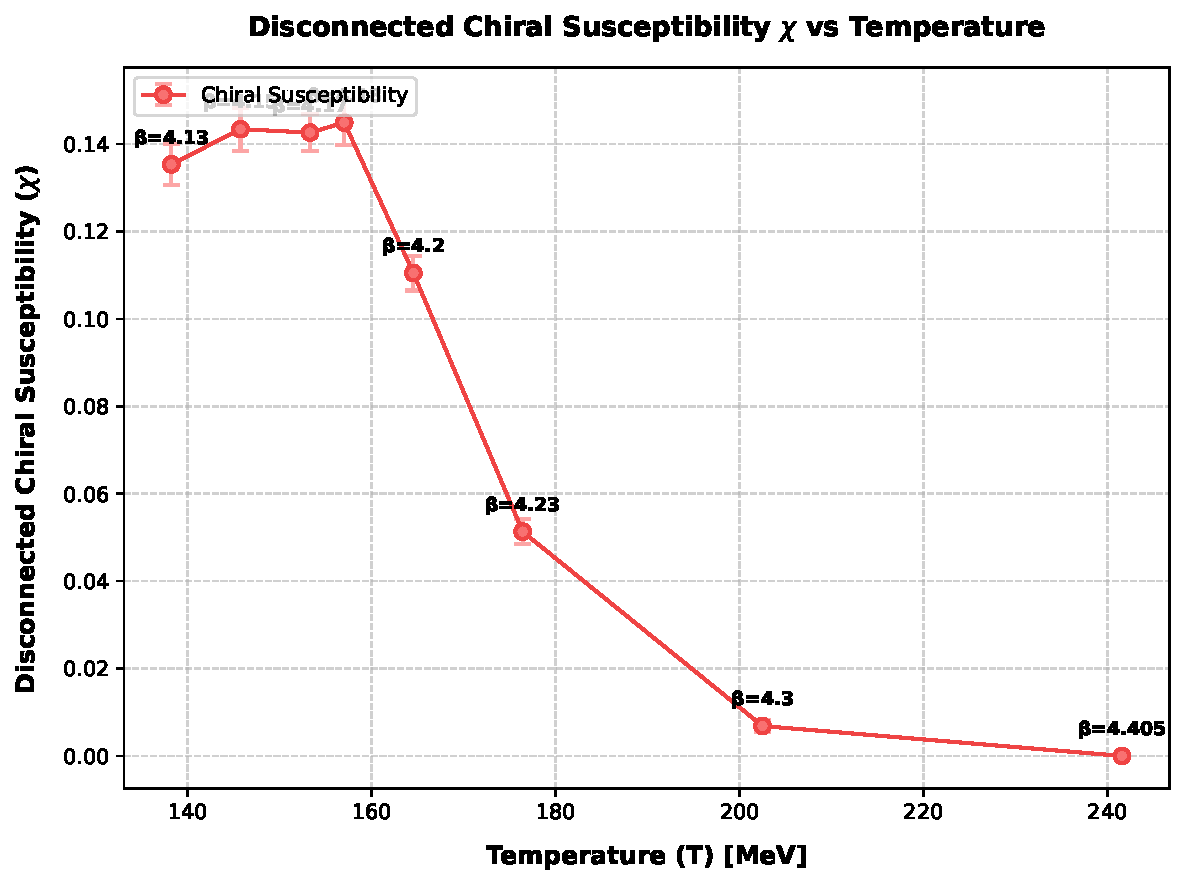
\includegraphics[width=0.82\textwidth]{docs/figures/sucep_plot.pdf}
    \caption{Four-dimensional volume-scaled chiral susceptibility $\chi_{\text{vol}} = N_s^3 N_t \chi$ as a function of temperature $T$ [MeV] for $48^3 \times 16$ lattices.}
    \label{fig:sucep_plot}
\end{figure}

\vspace{0.5cm}
\begin{center}
\small\textcolor{themegray}{--- End of Data Summary Report $\cdot$ ParseLQCData Framework ---}
\end{center}

\end{document}
